\chapter{Proposta de solução}

Neste capítulo serão apresentados os componentes e procedimentos utilizados na elaboração da proposta de solução, denominada ``BURI''. Conforme as
etapas definidas na metodologia, ocorre inicialmente a discussão sobre a fase de pesquisa na Seção \ref{fase1}, seguida pela especificação 
das funcionalidades e comportamento do sistema BURI, contextualizados na Seção \ref{fase2}. O particionamento e execução de atividades nas áreas de 
\textit{hardware} e \textit{software} são explicados nas Seções \ref{fase3} e \ref{fase4}, respectivamente. Na Seção \ref{fase5},  o aplicativo Android e o 
dispositivo físico são avaliados por um grupo selecionado de alunos, a fim de garantir a usabilidade do sistema proposto e, posteriormente, são produzidas a documentação 
do projeto e guia de instalação na Seção \ref{fase6}. 

\section{Pesquisa}\label{fase1}

A primeira fase consiste na compreensão do problema. O objetivo é encontrar trabalhos semelhantes sobre o uso de IoT no monitoramento da qualidade do ar, assim 
como as consequências fisiológicas de inalação prolongada de monóxido de carbono, e identificar, através de um questionário aplicado aos alunos, as preocupações relacionadas 
ao tema no ambiente doméstico.

Em primeiro lugar, realizou-se uma revisão da literatura para identificar pesquisas no âmbito de tecnologias IoT e monitoramento do ar com foco 
em prevenção de acidentes, porém foram selecionados cinco trabalhos acadêmicos para o desenvolvimento da proposta e comparação de funcionalidades. 
Além disso, o estudo da intoxicação por monóxido de carbono visa investigar as consequências para a saúde humana. Portanto, a explicação científica sobre o tema é do 
artigo ``Carbon monoxide poisoning: a review for clinicians'' \cite{carbon-monoxide-poisoning-varon}, pois o conteúdo inclui 
explicação técnica e didática do processo de envenenamento, consequências no sistema neurológico e cardiovascular, fontes de contaminação e métodos de tratamento utilizados na medicina.

Por fim, foi aplicado um questionário a um grupo de estudantes da Escola Superior de Tecnologia da Universidade do Estado do Amazonas (EST/UEA), para coletar informações acerca de suas
preocupações em relação à qualidade do ar no ambiente doméstico. A pesquisa teve como propósito identificar as características do ambiente residencial desses alunos e avaliar seu 
nível de conscientização sobre os riscos associados aos poluentes atmosféricos. Participaram deste levantamento inicial 58 estudantes matriculados em cursos da área de Engenharia, os quais responderam 
ao questionário de forma voluntária.

As respostas do questionário são relevantes para a construção do protótipo. Como destaque, algumas informações importantes serão analisadas a seguir. Segundo a pesquisa, 
75,9\% dos estudantes utilizam um \textit{smartphone} com 
Sistema Operacional Android, pois a tecnologia é fonte de acesso à informação e inclusão digital no Brasil \cite{impacto-android-brasil}. Outro aspecto analisado foi 
a percepção dos alunos em relação à qualidade do ar em suas residências e arredores. Nas respostas, os relatos sobre a presença de fumaça e dificuldade respiratória em dias específicos foram comuns. Como relatou um dos alunos: ``a fumaça se tornou um problema pra resolver isso decidimos comprar um umidificador de ar''. 

Evidência do problema apresentado, a Universidade do Estado do Amazonas (UEA) suspende atividades presenciais nos dias 19 e 20 de setembro na capital e interior por causa 
da alta quantidade de poluentes, pois os índices ultrapassaram a marca de 125 $\mu m/m^{3}$ e um ar de boa qualidade permite a concentração de partículas em  até 25 $\mu m/m^{3}$ \cite{uea-queima-fecha}. Portanto, 
o funcionamento de um dispositivo de medição em tempo real com interface para dispositivo móvel representa uma boa alternativa para auxílio do usuário.

\begin{figure}[ht]
    \centering
    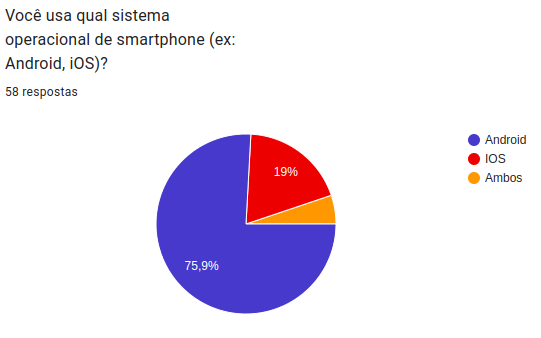
\includegraphics[width=.67\textwidth]{img/graf1-SO-smartphone.png}
    \caption{Sistemas Operacionais dos \textit{smartphones} dos alunos da EST. Fonte:Autor}\label{figSOsmartphone}
\end{figure}

Sobre o tipo de conexão com a internet, a Figura \ref{figWifiAlunos} ilustra a porcentagem de estudantes com rede Wi-Fi em suas residências. De acordo com a pesquia,  
a maioria dos entrevistados possui acesso à rede Wi-Fi. Esse valor é especialmente útil para a viabilidade do projeto, uma vez que a conectividade permitirá o funcionamento do sistema no modo \textit{online}.

\begin{figure}[ht]
    \centering
    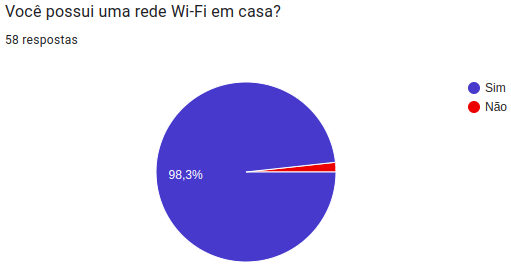
\includegraphics[width=.67\textwidth]{img/graf1-wifi.png}
    \caption{Uso de Wi-Fi dos alunos da EST. Fonte: Autor.}\label{figWifiAlunos}
\end{figure}

O último levantamento refere-se às expectativas em relação ao \textit{hardware}, destacando a preocupação com o uso do equipamento. Observou-se que apenas 37,9\% dos 
alunos já utilizaram algum dispositivo de automação residencial. Dessa forma, a solução proposta deve priorizar configurações simples, voltadas para usuários 
sem experiência prévia. 


\section{Especificação}\label{fase2}

A especificação é a etapa onde são definidas as funcionalidades do sistema embarcado e a modelagem da arquitetura e comunicação entre 
seus componentes. A partir das respostas, foram identificadas as principais funcionalidades 
para o sistema BURI, pois o desenvolvimento do sistema deve garantir que o protótipo final atenda às demandas reais do
público alvo. A funcionalidade de monitoramento em tempo real recebeu o maior número de votos (89,7\%) entre os participantes, porém opções como alerta de risco, fácil instalação e 
manutenção mínima foram requisitos proporcionalmente solicitados no questionário. 

\begin{figure}[ht]
    \centering
    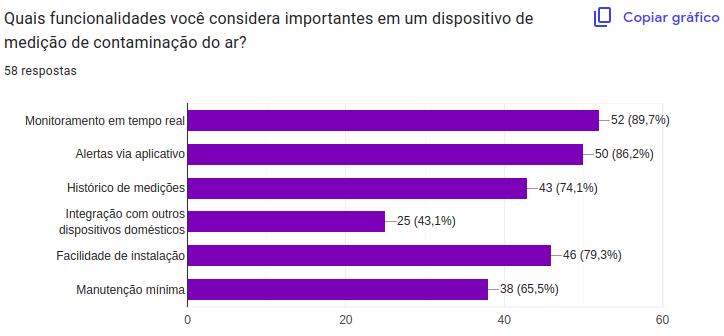
\includegraphics[width=.77\textwidth]{img/graf1-funcionalidades.png}
    \caption{Funcionalidades desejadas do sistema embarcado. Fonte: Autor.}\label{figFuncionalidades}
\end{figure}

Com base nas sugestões dos estudantes e considerando o prazo de entrega do trabalho de conclusão de curso, o escopo da proposta de solução contempla a 
implementação das seguintes funcionalidades: modo \textit{online} e \textit{offline}, monitoramento em tempo real, alerta de risco por notificação e processo de instalação facilitado.
As funcionalidades apresentadas têm o objetivo de equilibrar a expectativa dos usuários com a viabilidade técnica, pois a estrutura considera os recursos disponíveis e o prazo definido no 
cronograma.

O próximo passo da especificação é a modelagem de arquitetura do sistema, e para isso o projeto usa o padrão C4-model \cite{c4-model}. O C4 é um conjunto de ferramentas visuais usado pelo 
desenvolvedor de software na comunicação da arquitetura do sistema, semelhante a um mapa, com quatro níveis de detalhamento: \textit{context}, \textit{container}, \textit{component} e \textit{code}. A Figura \ref{figContextDiagram} é o 
diagrama de contexto, por mostrar a comunicação via protocolo HTTP ou Blueetooth do usuário doméstico com a aplicação. A implementação do sistema tem como serviço externo a ferramenta Ngrok \cite{ngrok}, pois o uso do túnel HTTP e \textit{link} estático permite a API do \textit{backend} ser acessível tanto pelo equipamento 
embarcado quanto pelo aplicativo Android na internet.

\begin{figure}[ht]
    \centering
    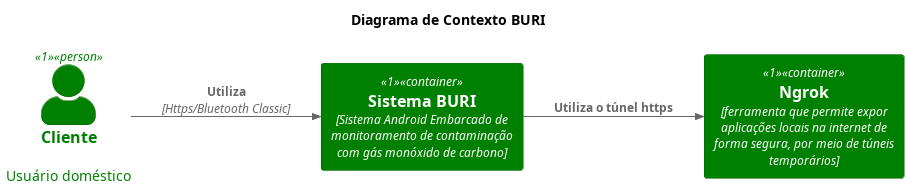
\includegraphics[width=.87\textwidth]{img/context-diagram.png}
    \caption{Diagrama de contexto. Fonte: Autor.}\label{figContextDiagram}
\end{figure}

O próximo diagrama é o de \textit{container}. Seu propósito é demonstrar o funcionamento da aplicação em termos de contêineres, ou seja, os elementos implantáveis
e componentes de software necessários para o pleno funcionamento do projeto. Na área de desenvolvimento de \textit{software}, o projeto possui três módulos principais: servidor, 
aplicativo e banco de dados. O servidor cuida das regras de negócio, como cadastro de usuários, dispositivos e login, mas também tem responsabilidade no 
armazenamento de medições do equipamento embarcado, cujo resultado é base para registro de eventos extremos. A segunda parte é o aplicativo Android. O módulo é a interface do sistema com o usuário doméstico, pois todo o fluxo de informação entre os 
diferentes componentes são fonte de dados para a visualização no \textit{smartphone} do indivíduo.

Por último, o Banco de Dados é responsável por armazenar todas as informações do sistema de monitoramento. Os dados de medição são organizados por dispositivo, onde 
cada um realiza o monitoramento de temperatura, umidade do ar e concentração de monóxido de carbono. Além disso, a estrutura de dados é otimizada para registrar tanto eventos críticos quanto 
medições dentro dos parâmetros normais.

\begin{figure}[ht]
    \centering
    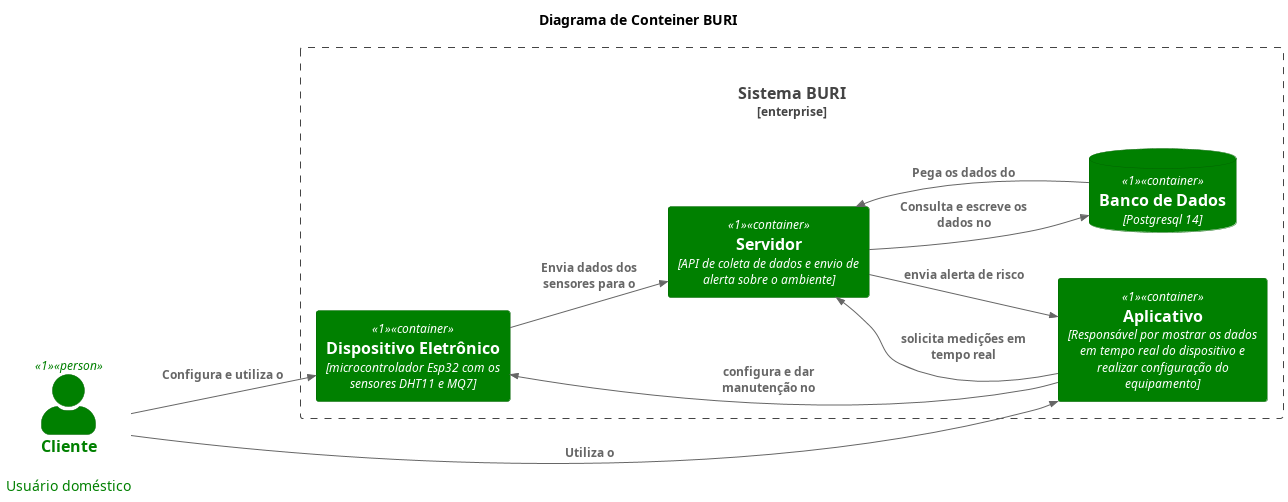
\includegraphics[width=.94\textwidth]{img/conteiner-diagram.png}
    \caption{Diagrama de container. Fonte: Autor.}\label{figConteinerDiagram}
\end{figure}

Sobre o \textit{hardware}, o sistema utiliza o dispositivo ESP32, juntamente com os sensores DHT11, para medição de temperatura e umidade do ar, e o MQ-7, para 
detecção de concentração de monóxido de carbono (CO). O microcontrolador atua no recebimento e envio de dados desses sensores e gerência da comunicação com o servidor ou aplicativo Android, mas seu funcionamento depende da energia da porta USB do 
notebook.

A próxima camada de abstração é o diagrama de componentes, no qual cada componente é responsável por um conjunto de tarefas bem definidas. Esses componentes interagem entre si por meio de interfaces ou contratos, 
garantindo a comunicação estruturada entre eles. A primeira representação é o diagrama de componentes do \textit{hardware}, pois ele detalha os sensores utilizados pelo microcontrolador, assim como 
os atuadores LED, usado na sinalização visual do modo de operação do circuito eletrônico, e o \textit{push button}, pois aciona a troca do modo de operação (\textit{online}/\textit{offline}) do dispositivo. Portanto, 
o \textit{hardware} também se comunica com o servidor e o aplicativo Android para envio de dados.

\begin{figure}[ht]
    \centering
    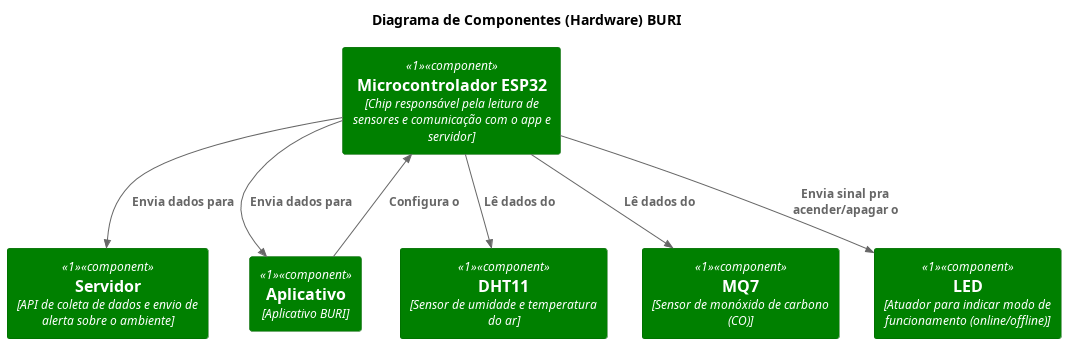
\includegraphics[width=.88\textwidth]{img/component-diagram-hardware.png}
    \caption{Diagrama de Componente (\textit{Hardware}). Fonte: Autor.}\label{figComponentHardware}
\end{figure}

Por último, será apresentado o diagrama de componentes do \textit{software}. O servidor tem acesso direto ao banco de dados e possui três principais controladores: \textit{Account Controller}, \textit{Measurement Controller} e \textit{Event Controller}. 

O primeiro gerencia os dados de usuário e seus dispositivos cadastrados, além de configurar o processo de autenticação e \textit{login} via dados de email e senha. Em seguida, o \textit{Measurement Controller} é interface de recebimento dos dados de cada dispositivo eletrônico, assim como 
o compartilhamento de informação com o aplicativo Android. O \textit{Event Controller} é o principal responsável na emissão de alerta de risco no aplicativo, pois o controlador recebe os dados em tempo real do banco de dados e avalia, 
com base em alguns parâmetros, se o ambiente possui comportamento perigoso, gerando o registro de um novo evento no banco de dados.

\begin{figure}[ht]
    \centering
    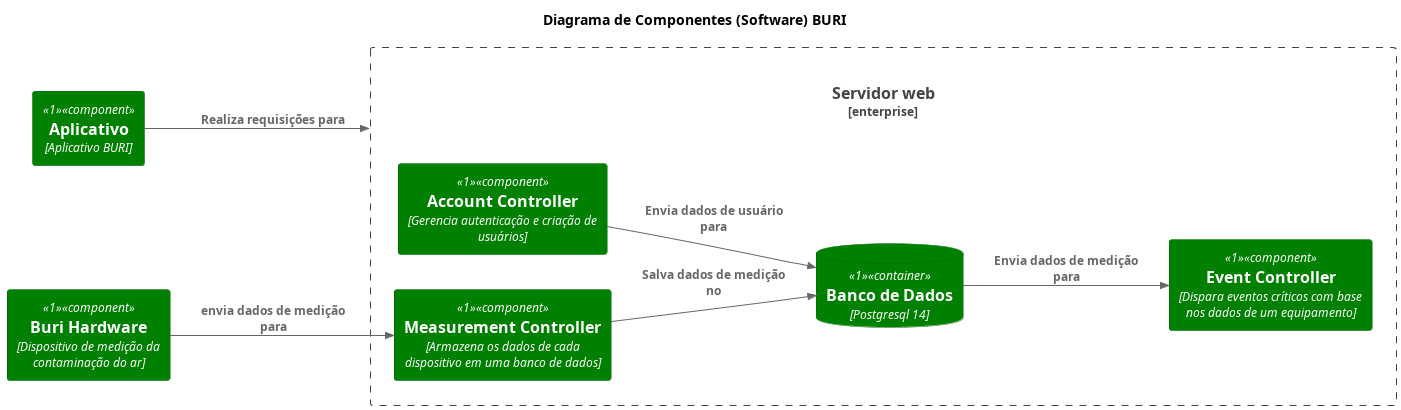
\includegraphics[width=.94\textwidth]{img/component-diagram-software.png}
    \caption{Diagrama de Componente (\textit{Software}). Fonte: Autor.}\label{figComponentSoftware}
\end{figure}

\section{Particionamento (Hw/Sw)}\label{fase3}

Após a conclusão da especificação, inicia-se o particionamento das atividades. Esse processo envolve a divisão do trabalho em tarefas menores, facilitando 
a organização, a alocação de recursos e a mensuração do progresso durante a fase de desenvolvimento. Portanto, as atividades de \textit{software} (Sw) são definidas de acordo 
com a lista a seguir.

\begin{itemize}
    \item Desenvolvimento da modelagem e implantação do Banco de Dados;
    \item Implementação da API:
    \begin{itemize}
        \item Rota de gerenciamento de conta de usuário;
        \item Rota de Medição em tempo real por dispositivo;
        \item Rota de Eventos do ambiente;
    \end{itemize}
    \item Desenvolvimento do Aplicativo Android;
    \item Codificação do \textit{firmware} no ESP32;
\end{itemize}

Além das atividades de \textit{software}, o particionamento abrange também as atividades relacionadas ao \textit{hardware} (Hw). Essas atividades focam na concepção, desenvolvimento e montagem dos componentes 
eletrônicos do sistema, garantindo os requisitos definidos na especificação. As atividades de \textit{hardware} são descritas a seguir:

\begin{itemize}
    \item Escolha e estudo dos componentes eletrônicos;
    \item Implementação do controle do LED por botão;
    \item Montagem do circuito e verificação de leitura dos sensores;
    \item Configuração dos modos \textit{online} e \textit{offline};
\end{itemize}

A construção da proposta é o resultado da junção entre as duas áreas. Porém, desenvolver o sistema embarcado 
na metodologia iterativo e incremental exige o conhecimento prévio da dependência de serviços entre as partes, assim como o uso de protocolos 
de comunicação do início ao fim do projeto. Dito isso, a Figura \ref{figTarefasMetodologia} ilustra a organização das tarefas de HW e SW, considerando 
a integração entre os componentes logicamente dependentes dentro de cada iteração.

\begin{figure}[ht]
    \centering
    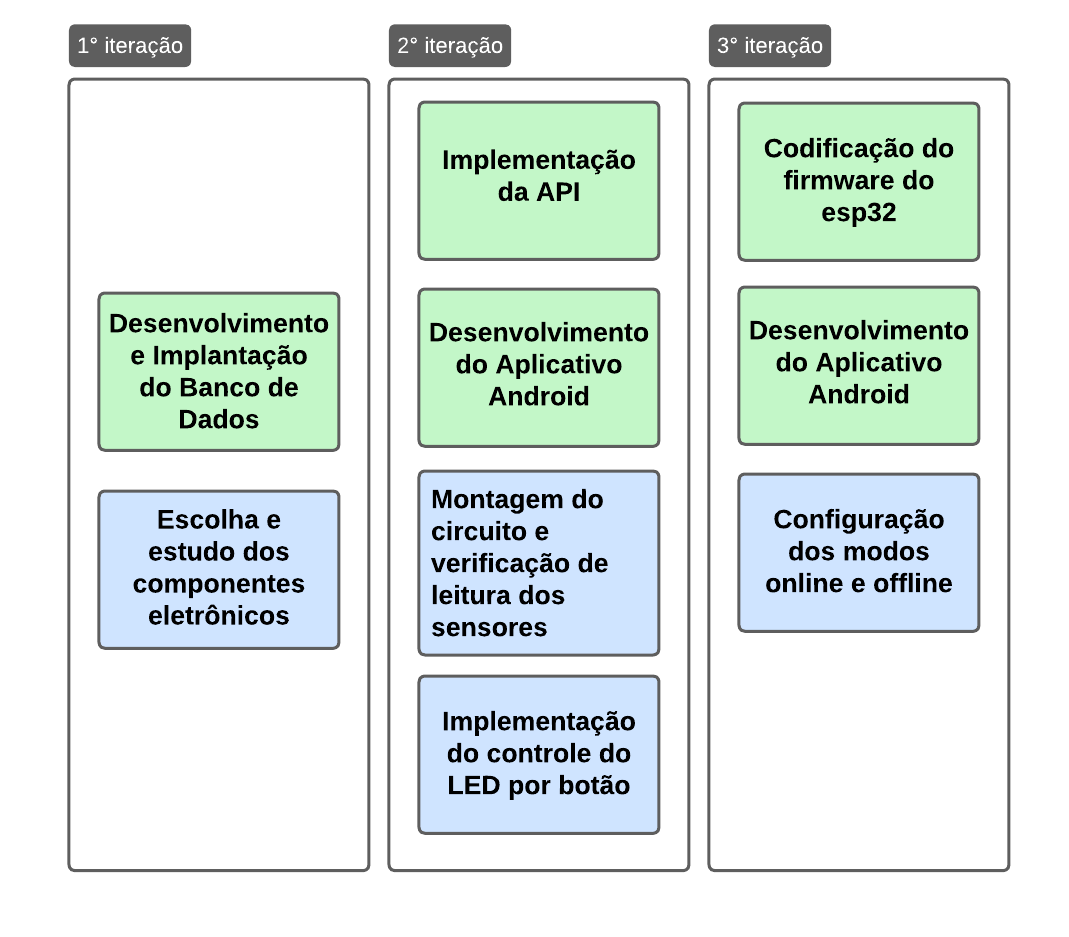
\includegraphics[width=.44\textwidth]{img/tarefas-metodologia.png}
    \caption{Organização de tarefas. Fonte: Autor.}\label{figTarefasMetodologia}
\end{figure}

\section{Execução de Atividades}\label{fase4}

Esta seção tem em vista detalhar os procedimentos adotados para a execução das atividades estabelecidas na etapa anterior. O desenvolvimento 
integrado de \textit{hardware} e \textit{software} exige uma abordagem iterativa, na qual funcionalidades específicas de uma área são projetadas para interagir com 
a outra, garantindo o sucesso na implementação do sistema.

\subsection{Primeira iteração}\label{ExecAtv1It}

A primeira atividade de \textit{software} diz respeito ao Banco de Dados, pois as informações de toda a aplicação 
precisam de registro e persistência. ``Um banco de dados representa algum aspecto do mundo real, às vezes chamado de minimundo ou de universo de discurso'' \cite[pp. 3]{banco-de-dados-navathe2014}. Assim como na engenharia de \textit{software}, o projeto 
de um banco de dados surge na análise de requisitos, pois nela são definidas as restrições e propriedades de cada conceito do mundo real cuja abstração 
deve ser persistida para futuras consultas. Portanto, o sistema BURI utiliza o Banco de Dados relacional \textit{PostgreSQL} e implementa a construção de tabelas 
via ORM (do inglês, \textit{Object Relational Mapper}), pois é uma técnica que permite o mapeamento dos objetos com os dados armazenados no sistema de banco de dados \cite{hibernate-documentation}. 

\begin{figure}[ht]
    \centering
    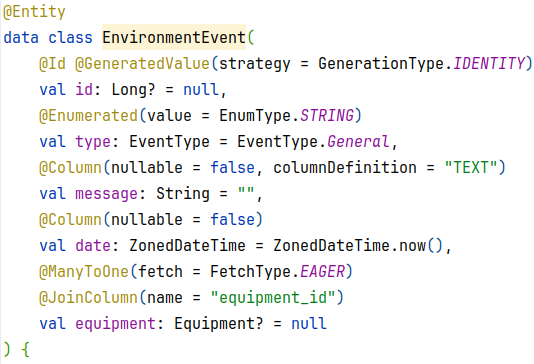
\includegraphics[width=0.45\textwidth]{img/event-class-kotlin.png}
    \hfill
    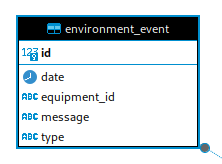
\includegraphics[width=0.42\textwidth]{img/event-table-postgres.png}
    \caption{Mapeamento Objeto Relacional da classe Evento. Fonte: Autor.}\label{figJpaEvent}
\end{figure}

Por outro lado, o \textit{Java Persistence API}, também conhecido pela sigla JPA, é uma camada 
de abstração do \textit{framework} para persistência de dados \cite{spring-data-jpa-documentation}. Seu papel 
é simplificar a operação com banco de dados relacionais, pois os desenvolvedores de \textit{software} utilizam objetos Java 
em vez de instruções SQL diretamente. Além disso, o projeto define um padrão de mapeamento de objetos para tabelas com base em anotações e
oferece recursos avançados de consulta via implementações do padrão de projeto \textit{Repository}. O esquema de Banco de Dados resultou na criação das 
tabelas e relacionamentos ilustrados na Figura \ref{figSchemaBuriDB}.

\begin{figure}[ht]
    \centering
    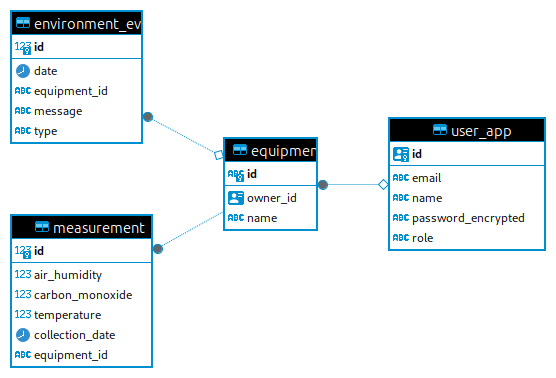
\includegraphics[width=.54\textwidth]{img/buri_schema_bd.png}
    \caption{Esquema do Banco de Dados BURI. Fonte: Autor.}\label{figSchemaBuriDB}
\end{figure}

No modelo, o usuário pode obter vários dispositivos e cada dispositivo tem a responsabilidade de atualizar as tabelas de medição e evento 
a partir da conexão por Wi-Fi com o servidor. Porém, o servidor possui uma rotina de verificação da medição atual antes de inserir no banco de dados 
para o sistema poder identificar se os valores registrados correspondem a um evento crítico ou não. 

A atividade de \textit{hardware} desta etapa consiste na pesquisa e estudo dos componentes eletrônicos. Conforme as variáveis de interesse deste trabalho de 
conclusão de curso, os sensores de medição escolhidos foram o DHT11 e o MQ-7, os mesmos utilizados no trabalho acadêmico \textit{AirWorld} \cite{UFAMAirWorld}. Uma vez definido os sensores, 
o próximo passo consiste na escolha do microcontrolador, pois ele será responsável por gerenciar as leituras dos sensores, processar os dados e comunicar-se com o servidor para armazenar as medições.

O ESP32 foi escolhido devido à sua versatilidade, ao possuir conectividade Wi-Fi e Bluetooth integradas, o que facilita a comunicação sem fio com outros componentes do sistema de monitoramento. Além disso, destaca-se 
pela robustez e poder de processamento, ao oferecer maior velocidade de processamento em comparação com outras opções, o que é essencial para o desempenho do sistema. Outro destaque é a economia, já que o microcontrolador 
é relativamente acessível, quando comparado a outras placas de desenvolvimento com funcionalidades semelhantes, tornando-o ideal para o desenvolvimento rápido de aplicações, pois a análise da Figura \ref{figTableEsp} fundamenta a decisão.

Em seguida, foi realizada a aquisição dos materiais necessários para o desenvolvimento do projeto, incluindo os sensores, o microcontrolador e outros componentes eletrônicos essenciais para a implementação do circuito. A compra dos itens 
otimizou os recursos financeiros e atendeu às especificações técnicas do projeto embarcado. Para tanto, são apresentados a seguir os custos da solução proposta na Tabela \ref{tabPrecoHardware}.

\begin{table}[h!]
    \centering
    \caption{Custo total de componentes eletrônicos para a prototipação do \textit{hardware}. Os preços são de lojas em Manaus no período de abril a julho de 2024. Fonte: Autor.}\label{tabPrecoHardware}
    \begin{tabular}{c|c|c}
        \hline
        \textbf{Quantidade} & \textbf{Nome do componente} & \textbf{Custo R\$} \\
        \hline
        1 & DHT11 - Sensor de umidade e temperatura & 15,50 \\
        \hline
        1 & MQ-7 - Sensor de monóxido de carbono & 32,00 \\
        \hline
        1 & WROOM-32 ESP32S - 30 Pinos & 58,00 \\
        \hline
        1 & Resistor 30 Ohms 5\% & 0,20 \\
        \hline
        1 & Resistor 200 kOhms 5\% & 0,40 \\
        \hline
        1 & LED difuso verde 5mm & 0,40 \\
        \hline
        1 & Botão \textit{push button} chave táctil & 0,25 \\
        \hline
        10 & 1 Kit Jumper Macho-Fêmea & 5,00 \\
        \hline
        10 & 1 Kit Jumper Fêmea-Fêmea & 5,00 \\
        \hline
        10 & 1 Kit Jumper Macho-Macho & 5,00 \\
        \hline
        1 & Cabo de Dados USB V8 Micro USB & 9,50 \\
        \hline
        1 & Protoboard 400 furos & 15,00 \\
        \hline
        \textbf{--} & \textbf{Custo Total} & \textbf{146,25} \\
        \hline
    \end{tabular}
\end{table}

O DHT11 é um sensor com leitura digital comumente usado em projetos de automação para medição de temperatura e umidade do ar. O dispositivo 
tem quatro pinos: \textbf{VCC}, responsável pela alimentação do sensor (3.3V a 5V); \textbf{GND}, que conecta ao sinal terra de referência do circuito; \textbf{DATA}, onde ocorre a transmissão 
de dados digitais; e \textbf{NC}, um pino específico sem utilidade \cite{dht11-documentation}. Por conta de suas características, como a capacidade de fornecer leituras confiáveis em condições normais de ambiente, como 
temperatura de 0 a 50°C e umidade do ar na faixa de 20 a 90\%, ele é a solução ideal para a aplicação em ambiente doméstico do sistema de monitoramento da contaminação do ar.

O segundo sensor utilizado no projeto é o MQ-7, sensível à presença de monóxido de carbono (CO) e amplamente empregado em equipamentos industriais e automotivos. Ele possui quatro 
pinos, sendo dois deles (\textit{VCC} e \textit{GND}) destinados ao controle de energia e os outros dois à leitura de dados, sendo o pino \textbf{AO} para valores analógicos e o pino \textbf{D0} para saídas digitais. 
O processo de calibração envolve a exposição do sensor a um ambiente limpo, seguido de um ambiente com concentração elevada de CO, para permitir o ajuste dos valores analógicos com a concentração de monóxido 
de carbono conhecida pela curva de resistência do dispositivo eletrônico \cite{mq7-documentation}.

\subsection{Segunda iteração}\label{ExecAtv2It}

A iteração atual concentra as principais atividades do desenvolvimento do projeto: implementação da API, 
desenvolvimento do aplicativo Android, montagem do circuito e leitura dos sensores, implementação do sistema de LED-botão. A API (Application Programming Interface) funciona como um contrato 
entre diferentes componentes de \textit{software}, permitindo a comunicação de dados e o compartilhamento de recursos. Por sua vez, o padrão 
arquitetural REST é um estilo para a construção de APIs que utiliza o protocolo de comunicação HTTP. Esse padrão usa verbos como 
GET, PUT, HEAD e DELETE para interagir com os recursos, identificados de forma única via URIs (\textit{Uniform Resource Identifiers}) \cite{api-definition}.

O servidor \textit{backend} do sistema embarcado é uma API REST construída sob o \textit{framework} Java Spring \cite{spring-boot-documentation}. A escolha 
do \textit{framework} baseia-se na recomendação do Google\textsuperscript{\textregistered} sobre o uso da linguagem Kotlin para desenvolvimento de aplicativos Android \cite{android-developers}.
O Kotlin é uma linguagem orientada a objetos, concisa e interoperável com a linguagem de programação Java \cite{kotlin-documentation}. Portanto, a característica \textit{full stack}, ou seja, a 
capacidade de construir aplicações completas, desde o servidor e banco de dados até o componente gráfico da solução (telas), motivou a adoção da linguagem Kotlin para o desenvolvimento do sistema BURI.

A primeira rota da API é a \textit{AuthResource}. Identificada pelo prefixo ``/auth'', sua função é realizar o cadastro de novos usuários 
do sistema e realizar a autenticação (login) com base nas credenciais de email e senha fornecidas no cabeçalho da requisição HTTP, assim como 
fornecer acesso para o dispositivo eletrônico salvar as medições obtidas no ambiente em questão. Por fim, o recurso \textit{generateId} consiste no \textit{endpoint} de geração 
automático de IDs de equipamentos, pois cada aparelho possui um identificador de 6 caracteres aleatoriamente escolhidos no conjunto de letras do alfabeto e números decimais. 

\begin{figure}[ht]
    \centering
    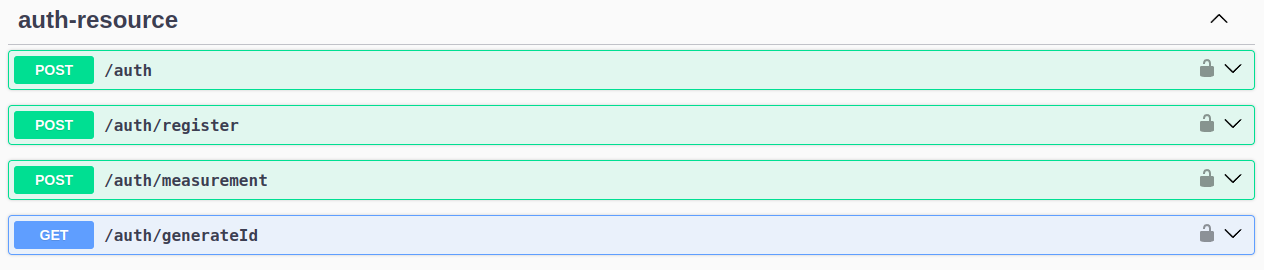
\includegraphics[width=.74\textwidth]{img/swagger-auth-resource.png}
    \caption{Rota de autenticação (\textit{Swagger Documentation API}). Fonte: Autor.}\label{figSwaggerAut}
\end{figure}

Após finalizada a etapa de autenticação da API, a próxima tarefa é implementar o código no aplicativo Android 
para realizar o cadastro e login na plataforma. Com o Android Studio, ambiente de desenvolvimento integrado oficial do Android, o projeto 
foi construído em módulos, sendo o \textit{package} data responsável pelo envio e tratamento de dados do aplicativo. Portanto, com o auxílio do cliente HTTP Retrofit \cite{retrofit}, 
a interface BuriApi implementou os métodos identificados na Figura \ref{figRetrofitAndroid}.

\begin{figure}[ht]
    \centering
    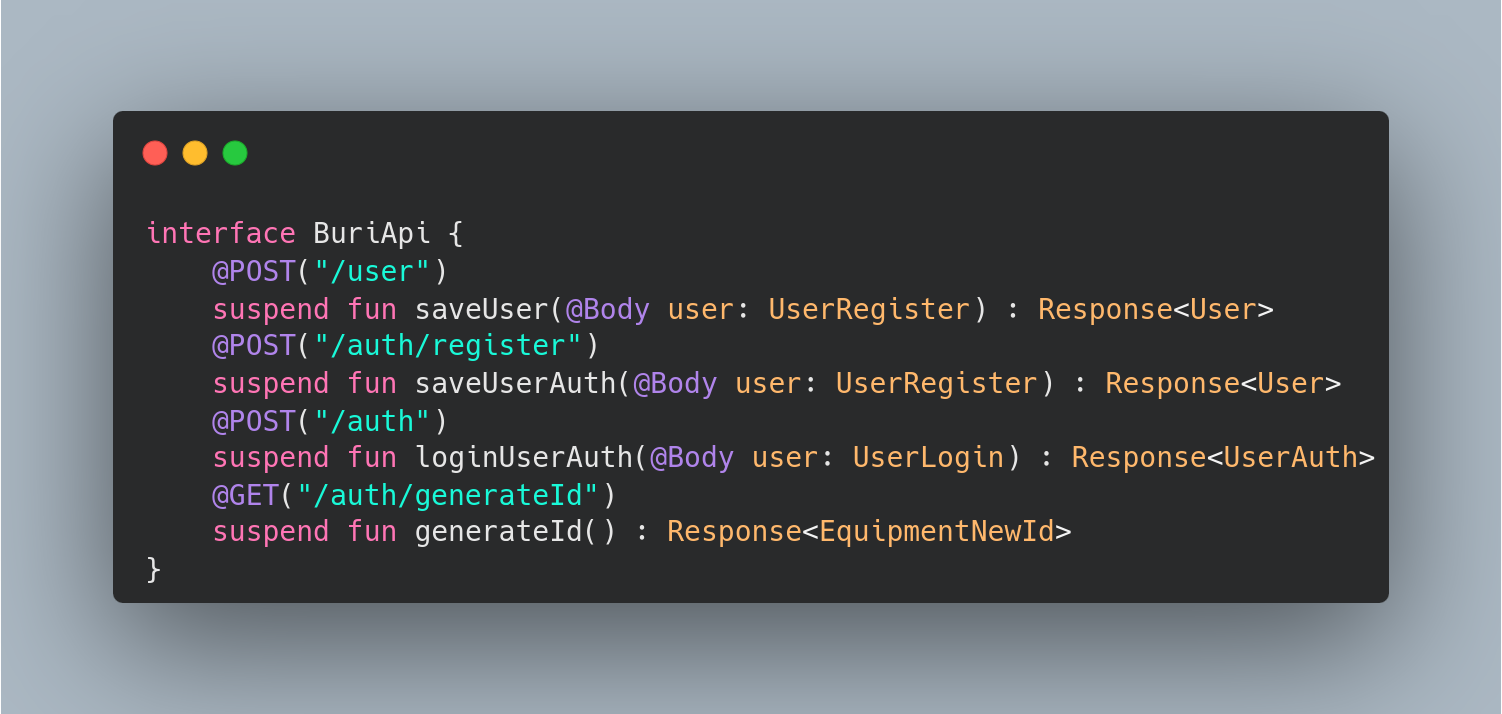
\includegraphics[width=.74\textwidth]{img/retrofit-buri-api-auth.png}
    \caption{Métodos de consumo da API no aplicativo Android. Fonte: Autor.}\label{figRetrofitAndroid}
\end{figure}

Em seguida realizou-se a implementação das seguintes telas do aplicativo: login, cadastro e lista de dispositivos. O aplicativo 
tem o propósito de facilitar a interação do usuário com a aplicação de monitoramento da contaminação do ar, pois ele se conecta 
tanto com o dispositivo quanto ao servidor via redes sem fio para mostrar dados em tempo real da concentração de monóxido de carbono. Como resultado das 
atividades realizadas, foi concluída com sucesso a primeira integração do sistema, conectando o servidor ao aplicativo Android nas 
funcionalidades de login e cadastro. 

Na área de \textit{hardware}, o circuito de troca do modo operacional é baseado no acionamento do \textit{push button}. Ao ser 
pressionado, o estado do dispositivo embarcado alterna entre os modos \textit{online} e \textit{offline}. O \textit{push button} 
tem duas configurações principais: normalmente aberto ou fechado. Essa diferença tem fundamento na estabilidade do nível lógico do botão 
quando não pressionado, pois, no caso de normalmente aberto o nível lógico é \textbf{ALTO} e muda para \textbf{BAIXO} no instante de acionamento \cite{arduino-docs}.

Ainda nessa tarefa, é preciso escrever o \textit{firmware} do ESP32 para interagir corretamente com o botão e o LED. O microcontrolador configura a 
leitura de GPIO via interrupção com o uso de uma variável global booleana (verdadeiro ou falso). Essa variável controla o fluxo de execução do programa principal 
e interage com LED, pois se o valor armazenado for verdadeiro, então o LED é ligado. A Figura \ref{figPushButtonFirmware} ilustra o trecho de código responsável pelo controle do modo operacional, onde a função principal 
executada pelo ESP é a \textit{loop}, porém a primeira função chamada é a \textit{setup}, cujo pino de leitura conectado 
no botão é definido como entrada de dados e, em seguida, associado a uma função de atualização da variável global do sistema. Por fim, a função \textit{loop} 
verifica o valor atual da variável através de uma estrutura condicional para execução de tarefas distintas. 

\begin{figure}[ht]
    \centering
    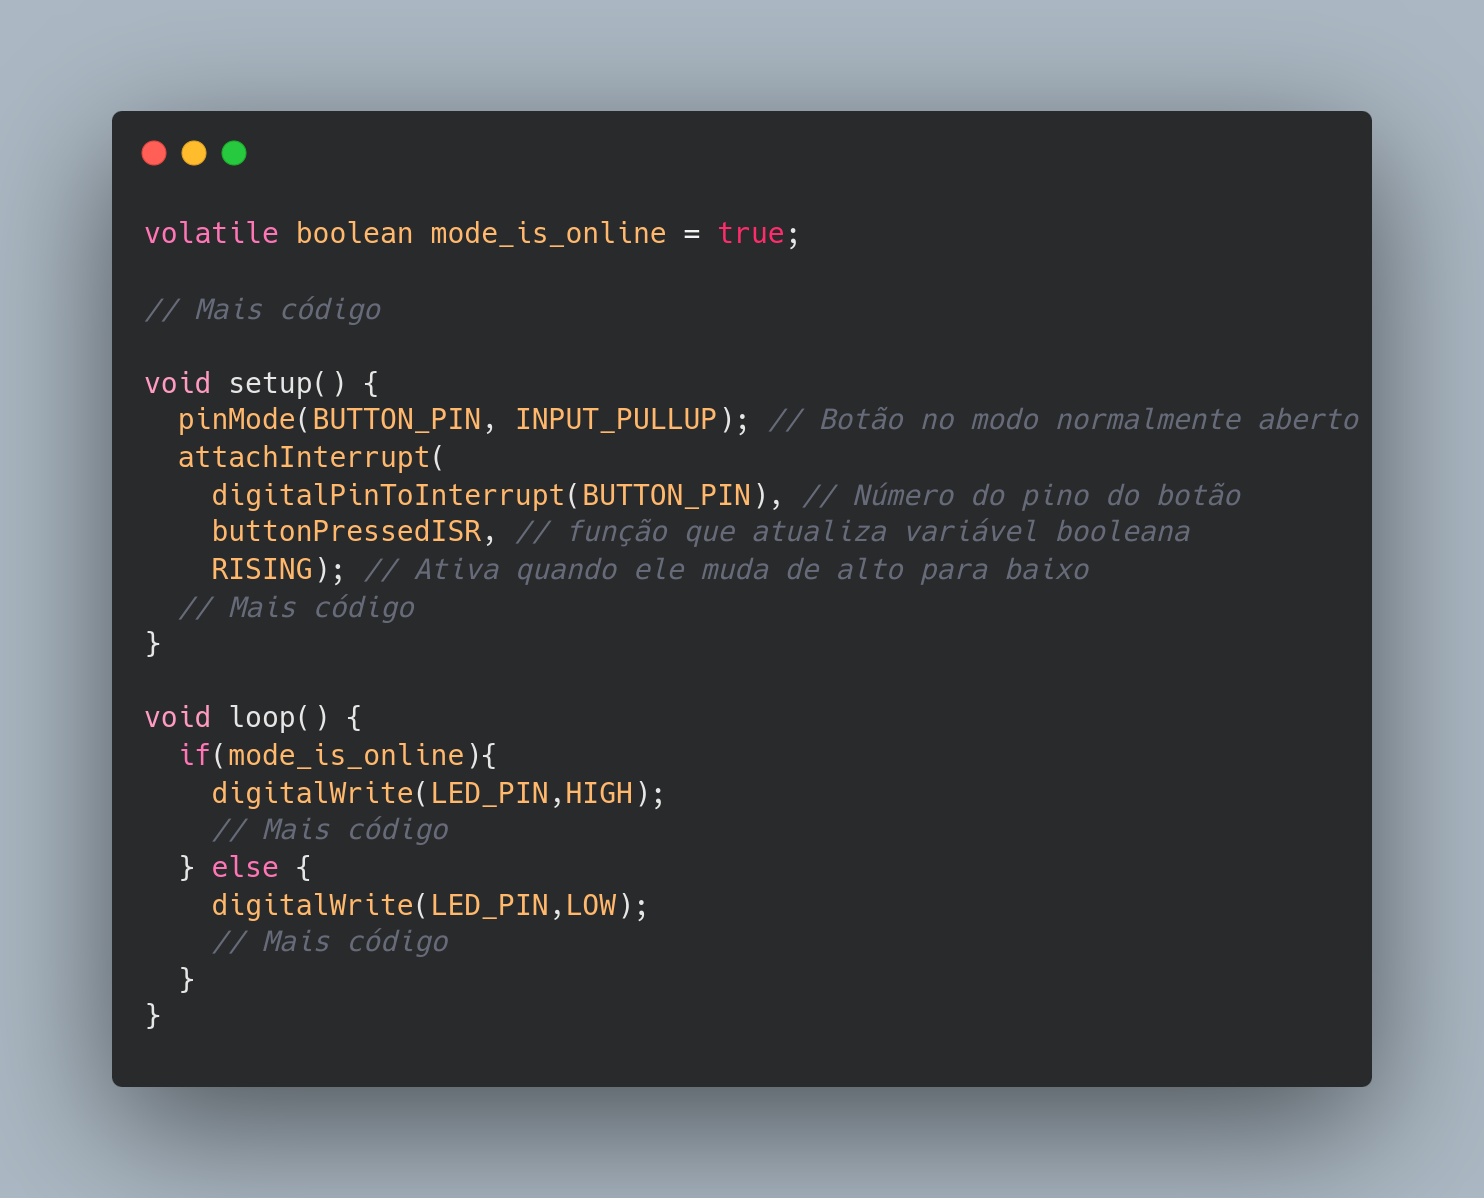
\includegraphics[width=.62\textwidth]{img/push-button-firrmware.png}
    \caption{\textit{firmware} para controle do LED e \textit{push button}. Fonte: Autor.}\label{figPushButtonFirmware}
\end{figure}

O próximo desafio do escopo de \textit{hardware} na segunda iteração é a montagem e leitura dos sensores DHT11 e MQ7. De acordo 
com as informações obtidas na Seção \ref{ExecAtv1It}, projetou-se o esquemático do circuito eletrônico formado pelo microcontrolador ESP32, sensores e conexões na matriz de contato. 
Após a modelagem, ocorre a montagem do dispositivo físico e a execução de programas individuais para leitura dos sensores, a fim de verificar a 
integridade das informações e o pleno funcionamento do protótipo. O ESP32 consome energia pela conexão Micro USB com a porta do notebook, pois 
no desenvolvimento do projeto os logs do microcontrolador são monitorados constantemente. 

\begin{figure}[ht]
    \centering
    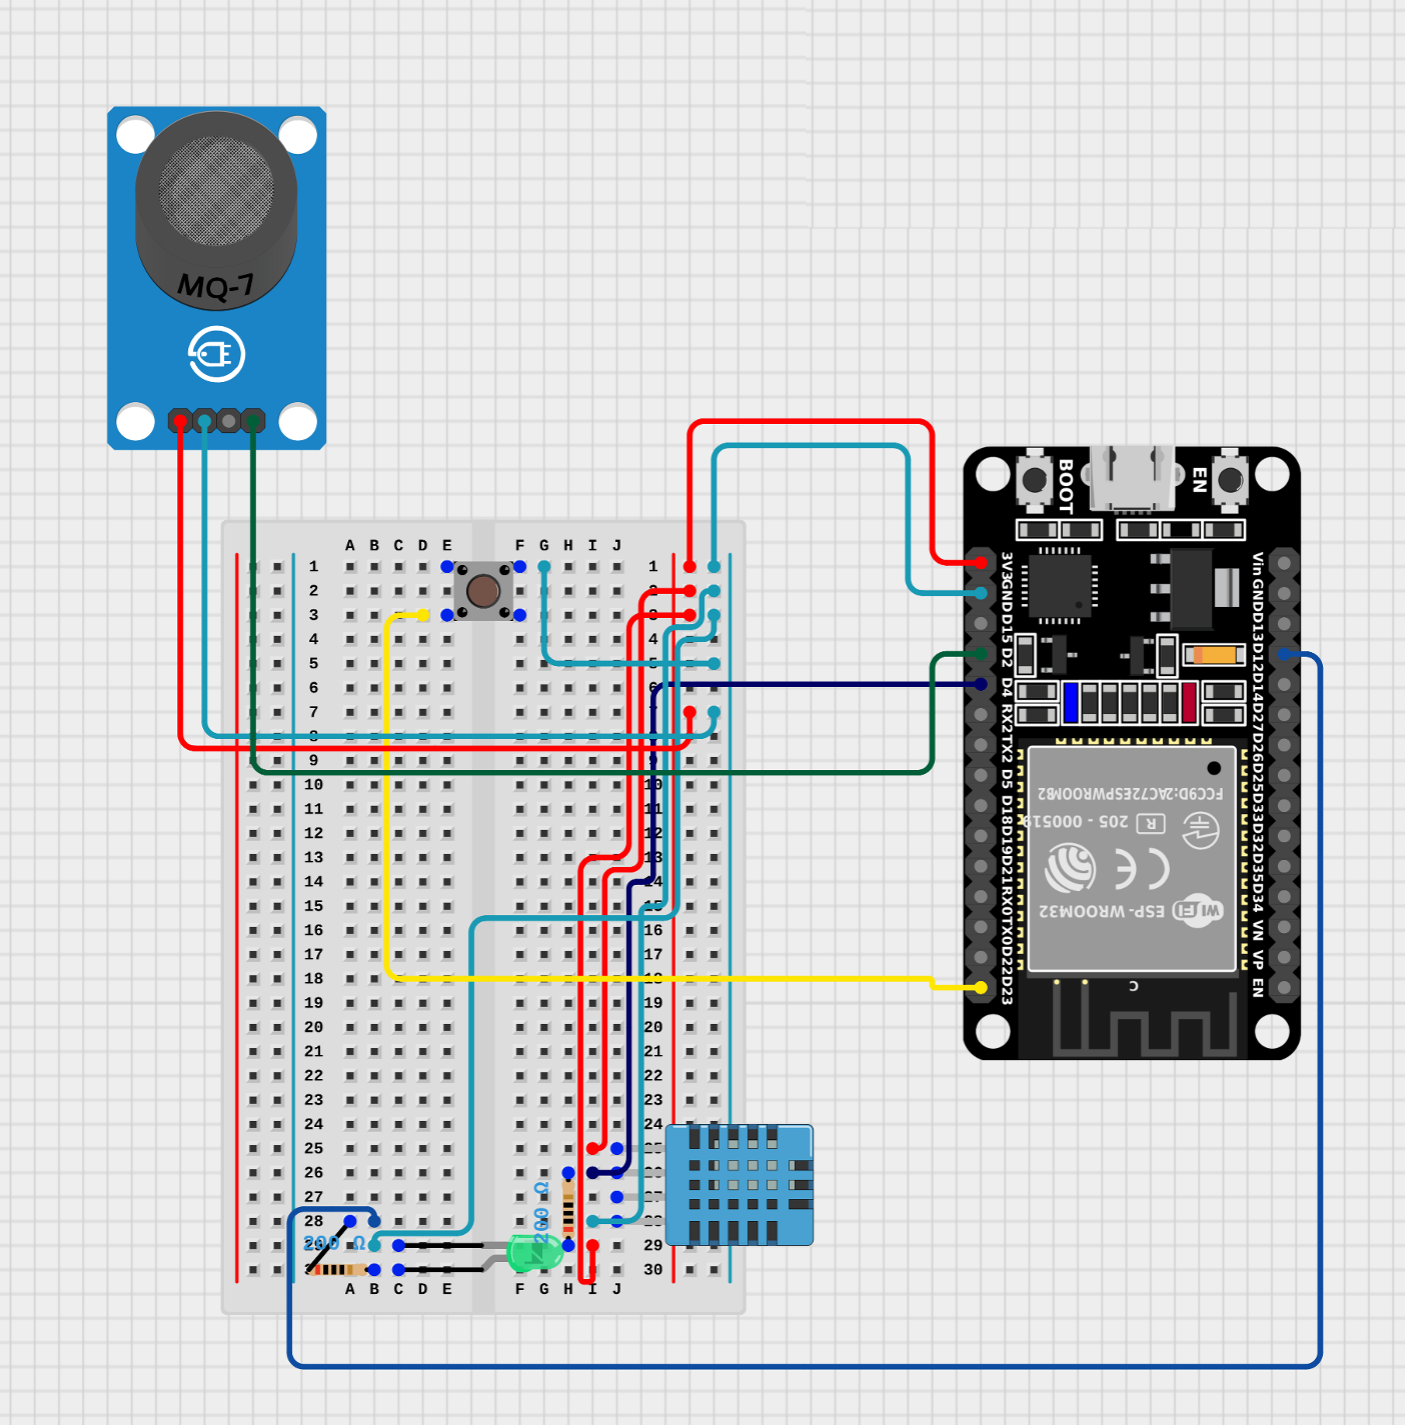
\includegraphics[width=.68\textwidth]{img/buri_esquematico.png}
    \caption{Esquemático do protótipo BURI \textit{Hardware}. Fonte: Autor.}\label{figSchematicBuriHardware}
\end{figure}

Por fim, a última atividade de \textit{software} termina com a implementação da API e publicação do servidor.  
Para o controle das medições, a rota ``/measurement'' recebe as informações de temperatura e umidade do ar, concentração de monóxido 
e id do equipamento, porém, antes de salvar no Banco de Dados, ocorre uma verificação no conjunto de dados para o envio de 
novos eventos do dispositivo. Por exemplo, a Tabela \ref{tabEfeitosCO} mostra os sintomas causados em seres humanos devido exposição ao 
monóxido de carbono.

\begin{table}[h!]
    \centering
    \caption{Sintomas de exposição ao monóxido de carbono. Fonte: Retirado de \cite{seguranca-contra-incendios}}\label{tabEfeitosCO}
    \begin{tabular}{p{4cm}|p{10cm}}
    \toprule
    \textbf{Concentração (PPM)} & \textbf{SINTOMAS} \\ \midrule
    35 & nenhum sintoma adverso dentro de 8 horas de exposição \\ \midrule
    200 & dor de cabeça após 2 a 3 horas de exposição \\ \midrule
    400 & dor de cabeça e náusea após 1 a 2 horas de exposição \\ \midrule
    800 & dor de cabeça, náusea e distúrbios após 45 minutos de exposição; morte em até 2 horas de exposição \\ \midrule
    1.000 & perda de consciência \\ \midrule
    1.600 & dor de cabeça, náusea e distúrbios após 5 a 10 minutos de exposição, perda de consciência após 30 minutos de exposição \\ \midrule
    12.800 & efeitos fisiológicos imediatos, perda da consciência e risco de vida após 1 a 3 minutos de exposição \\ \bottomrule
    \end{tabular}
\end{table}


Com base nas informações coletadas, o sistema de monitoramento avalia o estado atual do ambiente e registra um novo evento na 
tabela de Eventos, incluindo a mensagem de aviso correspondente. O aplicativo Android consulta regularmente o servidor para notificar 
o usuário sobre essas ocorrências. Entre as três variáveis monitoradas, o servidor prioriza os eventos relacionados ao monóxido de 
carbono, seguidos pela umidade e pela temperatura do ar, respectivamente, em uma mesma medição. 

O servidor disponibiliza os eventos via protocolo HTTP para o aplicativo realizar a consulta. A comunicação do servidor em ambiente local com os 
demais módulos da solução utilizou a ferramenta Ngrok \cite{ngrok}. Ngrok é um serviço que expõe aplicações 
locais à internet, ao criar endereço público com domínio personalizado sem a necessidade de contratar serviços de 
hospedagem para servidores em nuvem. Portanto, o código-fonte do aplicativo armazena o endereço público do servidor e o \textit{firmware} do microcontrolador 
ESP32 realiza a mesma ação, mas com o método de configuração específico para dispositivo embarcado.

\subsection{Terceira iteração}\label{ExecAtv3It}

Esta seção encerra o desenvolvimento do \textit{software} e \textit{hardware} do sistema de monitoramento da contaminação do ar. A primeira etapa consistiu na configuração 
do \textit{firmware}, o código executado no microcontrolador ESP32. Sobre a sua programação, o algoritmo estabelece dois modos de operação: o modo \textit{online}, que permite 
o envio de dados ao servidor por meio de uma conexão Wi-Fi, e o \textit{offline}, em que a comunicação ocorre diretamente com o aplicativo Android via rede Bluetooth.

O dispositivo de monitoramento requer conexão com a internet, um identificador único e acesso ao servidor. Para obter essas informações e estabelecer a interface com 
o usuário, utilizou-se a biblioteca Wifi Manager \cite{tzapu-wifimanager}, que possibilita a configuração das redes Wi-Fi via  portal de acesso configurável e acessível no navegador. Já para 
garantir a persistência dos dados durante as reinicializações do microcontrolador, foi utilizado a biblioteca de armazenamento SPIFFS Filesystem \cite{spiffs}. Essa solução permite armazenar
na memória \textit{flash} do ESP32 dados no formato de arquivo, de forma eficiente e organizada, permitindo que o dispositivo recupere as informações mesmo após desligamentos ou reinicializações inesperadas.

Em seguida, a próxima atividade de configuração é o envio de dados de ambiente para o servidor. O envio de dados foi implementado utilizando uma requisição HTTP no método POST, porém 
construída diretamente no código do microcontrolador. A URL da API (previamente configurada) foi recuperada da memória e durante o processo de construção da mensagem HTTP foram 
incluídos os cabeçalhos e o corpo da requisição contendo os dados coletados pelos sensores. No corpo da requisição, os seguintes valores foram adicionados: concentração de monóxido de carbono (ppm), umidade relativa do ar (\%), 
temperatura (°C), horário de coleta e identificador do equipamento cadastrado. Portanto, a Figura \ref{figPostMeasurement} ilustra a formatação da mensagem utilizando o protocolo HTTP.

\begin{figure}[ht]
    \centering
    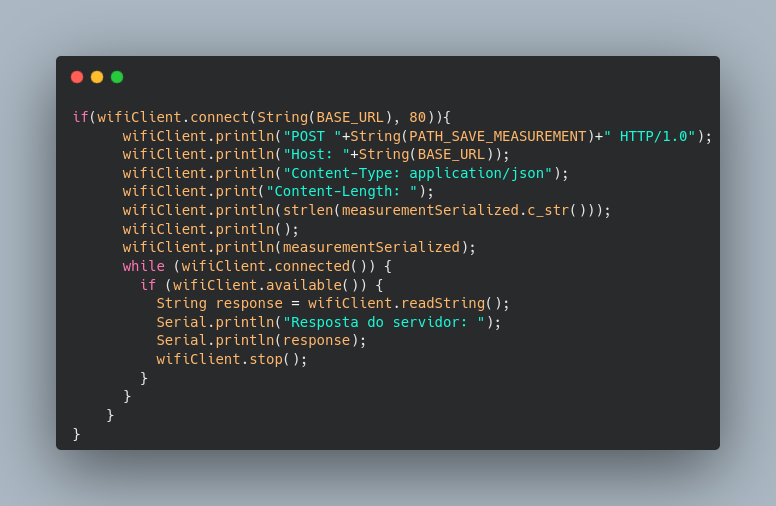
\includegraphics[width=0.53\textwidth]{img/POST-esp32-code.png}
    \hfill
    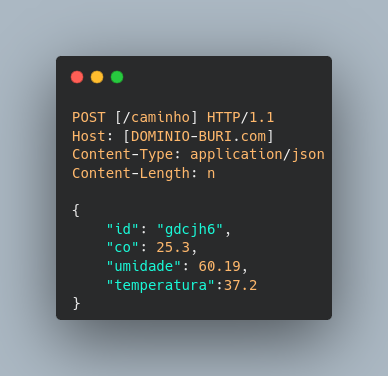
\includegraphics[width=0.36\textwidth]{img/POST-result.png}
    \caption{Código de envio e mensagem HTTP resultante. Fonte: Autor.}\label{figPostMeasurement}
\end{figure}

\section{Testes de aceitação}\label{fase5}

A etapa de testes de aceitação é o momento onde a aplicação desenvolvida sofre avaliação 
de usuários reais, cujo intuito é garantir que a solução atende aos requisitos e expectativas dos usuários finais ou \textit{stakeholders} \cite{system-design-IOT}. 
Portanto, dos 58 alunos entrevistados na fase de especificação, 38 participaram da avaliação de usabilidade do 
aplicativo BURI. O questionário foi enviado individualmente para os entrevistados por meio de aplicativo de comunicação após 
a execução das atividades práticas definidas no manual do sistema.

A análise de funcionalidade do sistema de monitoramento utilizou o SUS (\textit{System Usability Scale}) como abordagem para a elaboração de perguntas do questionário \cite{sus-design-questionario}. Desenvolvido por John Brooke, o método 
consiste em inserir perguntas com intervalo de 1 até 5 para indicar o grau de concordância da pessoa entrevistada com a afirmação descrita no escopo do texto. Porém, as perguntas originais foram adaptadas para contemplar o uso do sistema 
também na perspectiva do \textit{hardware} e sua comunicação com o dispositivo móvel, pois o projeto de sistemas embarcados abrange as duas áreas, \textit{software} e \textit{hardware}.

No que diz respeito às tarefas executadas na entrevista, o projeto BURI utiliza critérios e 
recomendações do livro ``\textit{A pratical Guide to usability testing}'' \cite{tarefas-design}. De acordo com os autores, estudos 
de usabilidade com impacto positivo estruturam um ambiente propício para coleta de dados qualitativos e quantitativos, ou seja, comentários escritos de participantes e 
graus em escala numérica para classificar a dificuldade na execução de tarefas. 

Portanto, o primeiro passo foi a criação do termo de consentimento livre com base no trabalho de Marilis (2022), porém adicionando preocupações sobre a saúde dos entrevistados 
em relação ao uso de sistema de monitoramento da contaminação do ar. Em segundo, ocorre a escolha das funcionalidades do sistema embarcado que serão alvo da pesquisa com os participantes, pois 
o documento de cenários de teste deve contextualizar o usuário a respeito de cada atividade \cite{tarefas-design}. Após isso, o manual de configuração e uso do sistema BURI é disponibilizado 
previamente aos participantes da avaliação prática, juntamente com o documento de cenários de teste. Esse procedimento permite ao entrevistado uma visão geral do que ele irá avaliar e também 
ajuda na familiaridade com o dispositivo embarcado.

O teste foi aplicado de forma presencial, em uma sala de aula da Escola Superior de Tecnologia da Universidade do Estado do Amazonas, onde foi possível utilizar o protótipo físico
e o aplicativo no ambiente controlado. Os estudantes foram divididos em grupos de 2 a 3 pessoas e instalaram o 
aplicativo no \textit{smartphone} via \textbf{apk}, formato de arquivo comum para distribuição de aplicativos Android \cite{android-developers}. Por limitação de tempo e apenas um exemplar do protótipo disponível, as 
tarefas escolhidas dentro das funcionalidades da aplicação são apresentadas na Tabela \ref{tab:cenarios-de-uso}. 

Conforme o objetivo geral deste trabalho de conclusão de curso, o sistema de monitoramento é direcionado a ambientes \textit{indoor}. Esses espaços são 
caracterizados por serem fechados, em contraste com ambientes externos ou ao ar livre, e por serem frequentemente ocupados por pessoas, como, por exemplo, escritórios comerciais. Assim, as atividades realizadas no ambiente de sala de aula 
buscam aproximar o projeto do contexto real e do público-alvo para o qual ele será efetivamente aplicado. Portanto, a Figura \ref{figTesteHardware} ilustra a aplicação de um dos testes 
com alunos de Sistemas de Informação e Engenharia de Computação.

\begin{table}[htbp]
    \centering
    \caption{Tarefas executadas no aplicativo BURI e suas respectivas descrições. Fonte: Autor, com base no estudo de \cite{ufam-design}.}\label{tab:cenarios-de-uso}
    \begin{tabular}{p{4cm}|p{10cm}}
    \toprule
    \textbf{Tarefa} & \textbf{Descrição} \\ \midrule
    Criar conta & Quando você acaba de instalar o app BURI, você quer realizar o cadastro na plataforma para acessar todos os dados sobre contaminação do ar em tempo real. \\ \midrule
    Realizar Login & Quando você é cadastrado e quer realizar o login no sistema BURI para ter acesso aos seus dispositivos e informações da sua residência. \\ \midrule
    Cadastrar novo dispositivo & Quando você tem um dispositivo eletrônico de medição de dados do ar, você quer cadastrá-lo na sua rede Wi-FI e no aplicativo para utilizá-lo e monitorar os dados em tempo real. \\ \midrule
    Visualizar Lista de dispositivos cadastrados & Quando você possui dispositivos cadastrados, você quer visualizá-los para escolher qual dispositivo você quer verificar os dados em tempo real. \\ \midrule
    Selecionar dispositivo & Quando você já escolheu o dispositivo que quer visualizar suas informações e integrar com o protótipo eletrônico. \\ \midrule
    Visualizar dados em tempo real (online) & Quando você seleciona o dispositivo que possui, você quer consultar as informações de temperatura, umidade do ar e concentração de monóxido de carbono, assim como o tempo em que foi realizada a coleta. Na versão online, você acessa um indicador visual que o sistema gera nesse modo eletrônico, que pode ser visualizado no protótipo eletrônico. \\ \midrule
    Visualizar dados em tempo real (offline) & Quando você seleciona o dispositivo que possui, você quer consultar os dados de temperatura, umidade do ar e concentração de monóxido de carbono no modo offline (usando conexão blueetooth). Nesse caso, você acessa apenas os dados já coletados e um indicador visual que o sistema gera nesse modo eletrônico. Pode-se possível alternar entre os modos. \\ \midrule
    Passar a propriedade de dispositivo eletrônico & Quando você já possui um dispositivo e quer passar ele para outra pessoa (já cadastrada no aplicativo) para que ela utilize no monitoramento da residência dela. \\ \bottomrule
    \end{tabular}
\end{table}

\begin{figure}[ht]
    \centering
    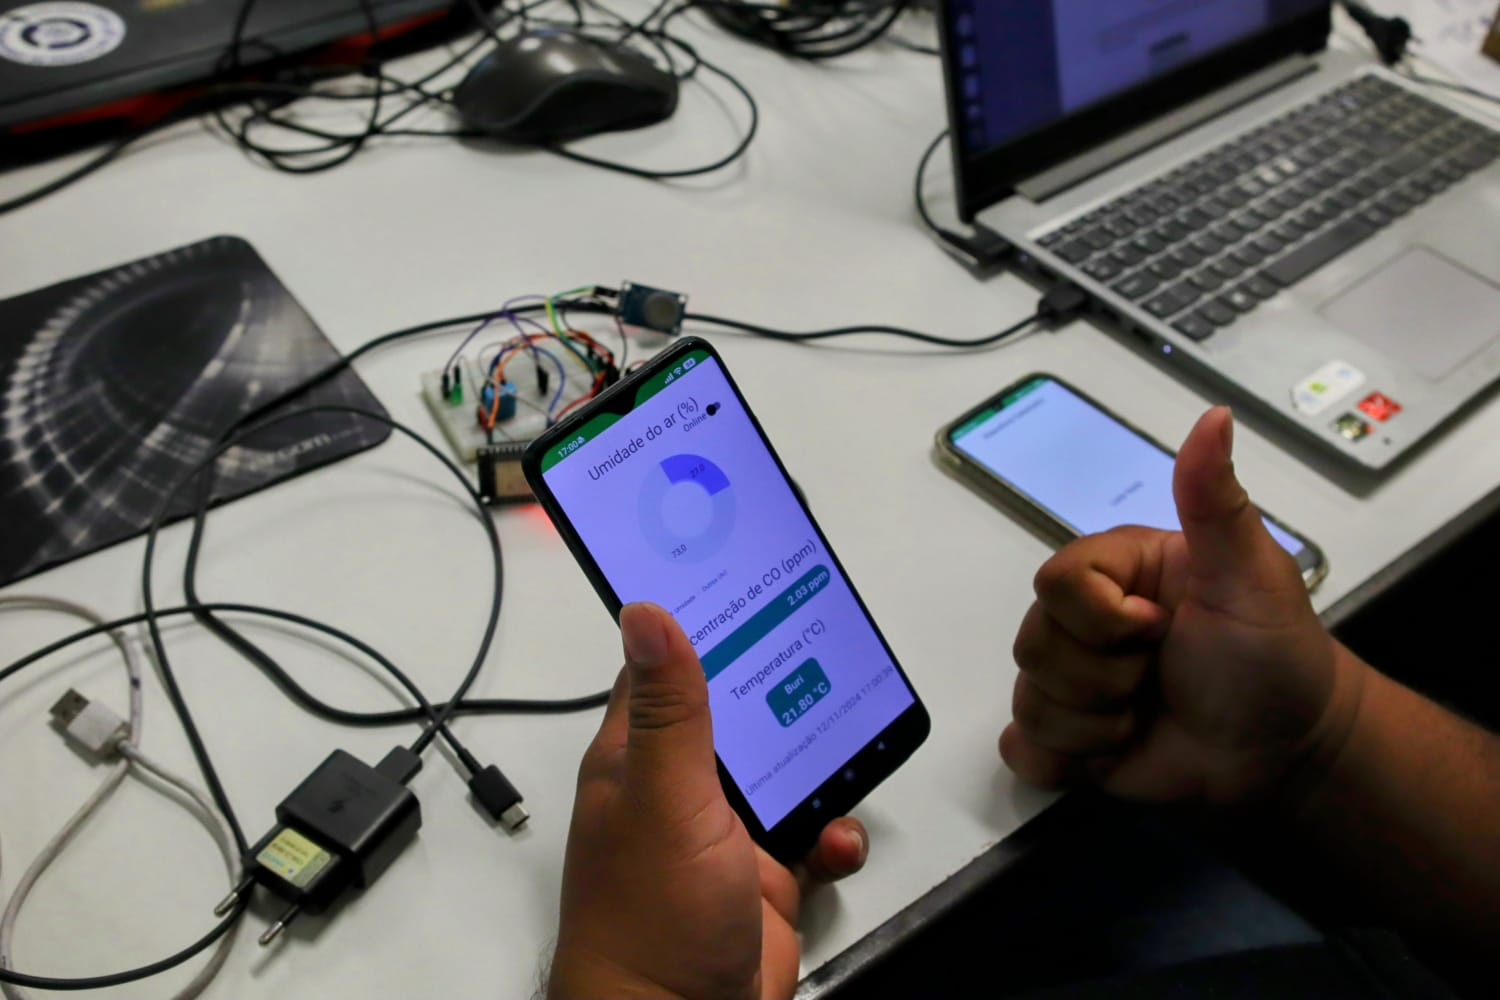
\includegraphics[width=.60\textwidth]{img/testes-praticos/hardware/testeBuriHardware1.jpeg}
    \caption{Teste de usabilidade do protótipo BURI. Fonte: Autor.}\label{figTesteHardware}
\end{figure}

\section{Documentação}\label{fase6}

O processo de documentação é fundamental para o compartilhamento e replicabilidade do projeto de sistema 
embarcado. Nesta fase, as informações são organizadas e registradas, abrangendo desde a descrição funcional do sistema até 
os procedimentos para instalação de dependências, pois o repositório remoto na plataforma de versionamento de código Github desempenha
a função de centralizar a documentação \cite{github}. Além disso, o projeto contém instruções detalhadas para a configuração de cada componente, 
incluindo a instalação e uso da API, o funcionamento do aplicativo e o processo de gravação do \textit{firmware} no dispositivo embarcado. Adicionalmente, 
ele também inclui o esquema eletrônico do hardware utilizado, bibliotecas de leitura de sensores utilizadas e, por último, orientações de instalação e exemplos de uso. 

Sobre organização de código, o repositório divide as linhas de desenvolvimento usando o conceito de \textit{branch}. Uma \textit{branch} (ou ramo) no sistema de versionamento GIT \cite{git-branch} é uma referência 
para um trecho de código e seu estado específico no tempo (\textit{commit}), servindo para realizar alterações pontuais sem comprometer o fluxo principal do repositório. Por exemplo, a \textit{branch} chamada 
``feat/api'' possui o código-fonte da API do servidor e todas as instruções técnicas para a execução da aplicação.

\begin{figure}[ht]
    \centering
    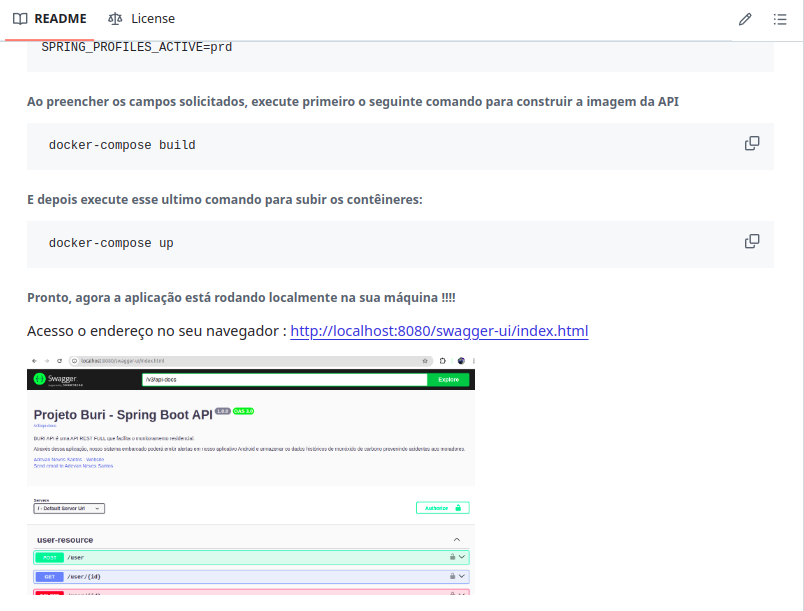
\includegraphics[width=.60\textwidth]{img/github-tcc-readme-api.png}
    \caption{Instruções para configuração da API. Fonte: Autor.}\label{figGithubAPI}
\end{figure}

Outro artefato relevante é o manual do sistema, elaborado visando atender às necessidades do usuário leigo. Esse documento foi estruturado em formato de tutorial, com uma linguagem clara e acessível, além de 
conter instruções detalhadas acompanhadas por imagens e pequenos textos explicativos. Ele abrange todo o processo de configuração e uso do dispositivo eletrônico, desde a instalação inicial até a troca de proprietário. Também 
orienta sobre como acessar e interpretar os dados por meio do aplicativo Android, garantindo que o usuário final utilize o sistema de forma autônoma. Porém, o manual foi responsável 
pela orientação das atividades do teste de aceitação, pois o guia serviu de consulta durante o experimento pelo grupo de alunos e, posteriormente, incorporado na fase de documentação.

\begin{figure}[ht]
    \centering
    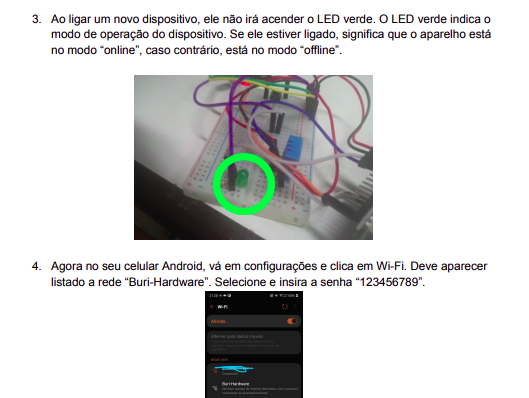
\includegraphics[width=.60\textwidth]{img/documentacao-manual.png}
    \caption{Manual do sistema BURI. Fonte: Autor.}\label{figGithubManual}
\end{figure}

A etapa final da documentação consolida o projeto como uma contribuição revelante e acessível para a comunidade. Como um sistema \textit{open source}, o código disponibilizado, dicas de uso e guias de instalação refletem a abordagem 
do trabalho para atingir desenvolvedores e usuários finais, interessados em expandir ou adaptar o sistema para outros contextos da área de IoT. Portanto, promove a democratização de soluções tecnológicas para melhorar a qualidade de 
vida das pessoas, assim como atua na prevenção de intoxicação por gás monóxido de carbono.
